\documentclass[format=acmlarge, review=false, nonacm=false, screen=true]{acmart}

\settopmatter{printacmref=false}
\renewcommand\footnotetextcopyrightpermission[1]{}
\pagestyle{plain}
\setcopyright{none}

\usepackage{hyperref}
\usepackage{minted}
\usepackage[utf8]{inputenc}
\usepackage{soul}
\graphicspath{ {./figures/} }
\makeatletter
\AtBeginEnvironment{minted}{\dontdofcolorbox}
\def\dontdofcolorbox{\renewcommand\fcolorbox[4][]{##4}}
\makeatother

\usepackage{color}

\DeclareRobustCommand{\hlcyan}[1]{{\sethlcolor{cyan}\hl{#1}}}

\begin{document}
\title{Plan/Proof of Concept: Visualizing the FWAE Language}

\author{Megha Singhania}
\affiliation{t4u0b@ugrad.cs.ubc.ca}
\author{Jonathan Chan}
\affiliation{r5x9a@ugrad.cs.ubc.ca}
\author{Samuel Or}
\affiliation{u4h1b, or.samuel1@gmail.com}
\author{Xuhao Chen}
\affiliation{d4i0b@ugrad.cs.ubc.ca}

\begin{abstract}
\vspace{0.75em}

Our project is of the fourth type: to create a substantial program in an esoteric language. It strives to produce an educational tool for the CPSC 311 course by providing parse tree and call tree visualizations, complete with environment and state illustrations, for the FWAE course language, which includes first-class functions but not mutation, laziness, or recursion. The parser and visualizer will both be implemented using Haskell, making use of the lazy and functional features of the language, as well as well-known libraries for parsing and visualization. We aim to complete up to the 90\%-level goal, which implements up to the parsing stage.
\end{abstract}

\maketitle

\setcounter{section}{-1}
\section{Introduction}
In this report, we will outline the parsing, interpretation, and visualization of the FWAE language from CPSC 311 using Haskell \cite{inclass6}. Section~\ref{parsing} will discuss parsing using monadic parser-combinators from the Parsec library \cite{parsec}, which is our 90\% goal, while section~\ref{interp-viz} will discuss interpretation of the parsed results and visualization of the parse and interpretation trees using the pretty-tree library \cite{pretty-tree}, which would be our 100\% goal. We are currently aiming for the 90\% level. Section~\ref{stretch} discusses further extensions and improvements beyond the 100\% goal.

All code snippets in this report can be found in the \texttt{fwae-parser} repository, which contains a rudimentary working implementation of the 90\% goal \cite{fwae-parser}.

\section{90\% Goal: Parsing}\label{parsing}
For the 90\%-level goal, we will implement a parser \hl{in Haskell for the FWAE language} \cite{fwae}. \hl{Various versions of this language is what is primarly used in CPSC 311; we will be using specifically the one defined in Chapter 6, "First-Class Functions".} 

\subsection{Preliminaries}
The EBNF we will use that describes the FWAE language is as follows:

\begin{minted}{ebnf}
<FWAE> :: <num>
        | <id>
        | {<op> <FWAE> <FWAE>}
        | {if0 <FWAE> <FWAE> <FWAE>}
        | {fun {<id>} <FWAE>}
        | {<FWAE> <FWAE>}
        | {with {<id> <FWAE>} <FWAE>}
<op>   :: + | - | *
<id>   :: (* begins with letter, rest are alphanumeric or `-` or `_` or `*` *)
          (* is none of `with`, `fun`, `if0`, `+`, `-`, `*` *)
\end{minted}

The Haskell data structures used to store the abstract syntax representation are similarly defined:

\begin{minted}{haskell}
data FAE = Number Double
         | Id     String
         | Op     OpType FAE FAE
         | If0    FAE FAE FAE
         | Fun    String FAE
         | App    FAE FAE
    deriving (Show, Eq)
data OpType = Add | Sub | Mul deriving (Show, Eq)
\end{minted}

They derive the \texttt{Show} and \texttt{Eq} typeclasses to allow printing in the REPL loop and to facilitate testing.

We will use the Parsec library for parsing \cite{parsec}. The first important structure we will encounter is a parser.

\begin{minted}{haskell}
-- defined by Parsec
data ParsecT s u m a
type Parsec s u = ParsecT s u Identity
-- defined by us
type Parser = Parsec String ()
\end{minted}

\texttt{ParsecT} is a monad-transformer "with stream type \texttt{s}, user state type \texttt{u}, underlying monad \texttt{m} and return type \texttt{a}" \cite{parsec-hackage}. Parsec provides a type alias \texttt{Parsec} to hide details we don't need to know about; similarly, we further define \texttt{Parser} to fix the input type as \texttt{String} and the state as \texttt{Unit} since we need not concern ourselves with it. The important part is what the parser returns, which will help us in combining parsers.

\subsection{Provided Parsers}

Now that we have a language syntax definition and parser type, we begin first by making an inventory of what parsers we have available. We can extend\footnote{Obviously, this is not extending in the OOP sense; here, we are creating a structure with the same fields as \texttt{emptyDef} but replacing only those fields we specify.} Parsec's empty language definition with just the restrictions we need to impose, then generate a structure containing parsers in it.

\begin{minted}{haskell}
fwaeDef = emptyDef {
    identStart    = letter, -- identifiers begin with any letter
     -- identifiers contain either an alphanumeric character or one of our allowed special characters
    identLetter   = alphaNum <|> oneOf "_-*",
    reservedNames = ["with", "fun", "if0", "+", "-", "*"] -- any special words used in the EBNF
}
lexer = makeTokenParser fwaeDef
\end{minted}

Conventionally, this is called a lexer since it contains the parsing tools we need to "[convert] a sequence of characters ... into a sequence of tokens" \cite{lexer}. For ease of reference, we extract the parsers inside \texttt{lexer} and annotate them with types.\footnote{To allow naming our own parsers the same, we import \texttt{Text.Parsec.Token} as \texttt{P}.}

\begin{minted}{haskell}
identifier = P.identifier lexer :: Parser String
reserved   = P.reserved   lexer :: String -> Parser ()
integer    = P.integer    lexer :: Parser Integer
whitespace = P.whiteSpace lexer :: Parser ()
braces     = P.braces     lexer :: Parser a -> Parser a
lexeme     = P.lexeme     lexer :: Parser a -> Parser a
float = lexeme sign <*> P.float lexer :: Parser Double
\end{minted}

What these parsers do should now be self-evident. \texttt{identifier} parses for a legal identifier and returns it; \texttt{reserved} parses for the reserved name we give it; \texttt{integer} parses for a signed integral number and returns it; \texttt{whitespace} parses for whitespacing, acting as a whitespace stripper. Less evident are \texttt{braces}, which parses for opening and closing braces, and applies the given parser on the interior of the braces; and \texttt{lexeme}, which applies the given parser and strips trailing whitespace. The \texttt{float} parser provided does not parse negative floats \cite{parsec-bug}, so we can create our own to do so, as above, following the implementation of \texttt{integer} \cite{token}.

\subsection{Combining Parsers}
To gain insight on how we might implement our core parser, we must first indicate how we might wish to use it. Of course, there must be some point at which we perform the actual application of a parser, using Parsec's \texttt{parse}.\footnote{This time, \texttt{PC} is the qualified import of \texttt{Text.Parsec}.}

\begin{minted}{haskell}
-- defined by Parsec
PC.parse :: Stream s Identity t => Parsec s () a -> SourceName -> s -> Either ParseError a
-- defined by us
parser :: Parser FAE
parse :: Parser FAE -> String -> Either ParseError FAE
parse =
    let helper = do
        whitespace      -- strip leading whitespace
        fae <- parser   -- extract the parse result
        eof             -- assert that the end of the input has been reached
        return fae
    in PC.parse helper ""
\end{minted}

The \hl{empty string argument corresponds to the \texttt{SourceName} parameter, which} "is only used in error messages and may be the empty string" \cite{parsec-hackage}. Our parser proper will be used recursively to parse subexpressions, so actions to be done at the start and end of the total input must be done here.

The most straightforward way to proceed is to define a separate parser for each branch of the EBNF. One may be tempted to naïvely combine them all with the \texttt{choice} combinator, which can be thought as a non-deterministic parser-picker.

\begin{minted}{haskell}
parser = choice [numberParser, idParser, opParser, if0Parser, funParser, appParser, withParser]
\end{minted}

The major pitfall here is that if a certain parser succeeds on the \textit{very first character}, the result of that parser will be used. This means that if we try to parse
\begin{minted}{haskell}
"{fungible fungiform}"
\end{minted}
which should be read as the application of the function bound to identifier \texttt{fungible} to the value bound to \texttt{fungiform}, \texttt{opParser} will see the opening brace and think that it can parse it, but ultimately fail because the next character, \texttt{f}, is not part of one of our operators. We then use Parsec's \texttt{try} on each of our parsers, which "behaves like [the given] parser \texttt{p}, except that it pretends that it hasn't consumed any input when an error occurs" \cite{parsec-hackage}.

\begin{minted}{haskell}
parser = choice $
    map try [numberParser, idParser, opParser, if0Parser, funParser, appParser, withParser]
\end{minted}

\begin{comment}
Some of the branches of the parser simply involve extracting a value from a parser and wrapping it in our data constructor. For instance, \texttt{idParser} would look like this:

\begin{minted}{haskell}
idParser = do
    id <- identifier
    return (Id id)
\end{minted}

The \texttt{numberParser} is implemented similarly\footnote{A technical detail: there must in fact be separate parsers for integers and floats due to how floats are defined in Haskell, but they follow the same principle.}. For branches wrapped in braces, we pass our parser to the \texttt{braces} parser combinator; our parser would look for a reserved word using \texttt{reserved}, then usually simply call upon \texttt{parser} recursively to parse subexpressions. For instance, parsing \texttt{if0} makes three recursive calls:

\begin{minted}{haskell}
if0Parser = braces $ do
    reserved "if0"
    cond <- parser
    on0  <- parser
    non0 <- parser
    return (If0 cond on0 non0)
\end{minted}
\end{comment}

The \texttt{numberParser} would parse any number \texttt{n} in the input and transform it into a \texttt{(Number n)}.
The \texttt{idParser} would parse any valid identifier \texttt{s} and transform it into an \texttt{(Id s)}.
\begin{minted}{haskell}
idParser = do
    id <- identifier
    return (Id id)
\end{minted}
The \texttt{opParser} would parse reserved operators, and transform them into their respective \texttt{Add}, \texttt{Sub}, or \texttt{Mul} form. Then it would parse the left and right expressions within.
The \texttt{if0Parser} would check for the reserved word \texttt{if0} and use the above parsers to parse its inner expressions.
The \texttt{funParser} would check that the reserved word \texttt{fun} is within braces, and parse the parameter in the inner braces using the \texttt{identifier} parser. Finally, we would parse the rest of the body recursively with one of the parsers above.
The \texttt{appParser} simply checks that it can be parsed as a function and parses the argument with one of the parsers above.
The \texttt{withParser} would check for the reserved word \texttt{with}, parse its name with the \texttt{identifier} parser, and parses the body recursively with a parser above.
\begin{minted}{haskell}
withParser = braces $ do
    reserved "with"
    (name, expr) <- braces (do
        name <- identifier
        expr <- parser
        return (name, expr))
    body <- parser
    return (App (Fun name body) expr)
\end{minted}
\hl{The \texttt{\$} function is function application; that is, \texttt{f \$ a} is equivalent to \texttt{f (a)}. The full implementation of each of these subparsers can be viewed on our repository} \cite{fwae-parser}.



\section{100\% Goal: Call Tree Visualization}\label{interp-viz}
\subsection{Part 1: Interpreting}
For the 100\%-level goal, we will implement the FWAE interpreter and the call tree interpreter \hl{, which will be used to extract the environment at each node of the abstract syntax tree}. Besides, we will visualize the call tree produced with metadata.
\subsubsection{Interpreter}
The interpreter of FWAE is implemented with Haskell as follows:
\begin{minted}{haskell}
data Value  = NumV Double | ClosureV String FAE Env deriving (Show, Eq)
data Env    = MtEnv | AnEnv String Value Env deriving (Show, Eq)

interp :: FAE -> Either String Value
interp fae = helper fae MtEnv
       where helper :: FAE -> Env -> Either String Value
             helper(Number n)        _   = Right $ NumV n
             helper (Op op lhs rhs)  env = do
                  leftVal  <- helper lhs env
                  rightVal <- helper rhs env
                  Right \$ execOp op leftVal rightVal
             helper (Id id)         env = lookupId  id env
             helper (Fun param body)env = Right $ ClosureV param body env
             helper (If0 cond on0 non0) env = do
                  condVal <- helper cond env
                  NumV n  <- isNumV if0NonNumErrorMsg condVal
                  helper(if n=0 then on0 else non0)
             helper (App fun arg)  env = do
                  funVal  <- helper fun env
                  argVal  <- helper arg env
                  ClosureV param body cenv <- isClosureV appNonClosureErrorMsg funVal
                  helper body (AnEnv param argVal cenv)
\end{minted}
In the helper functions above, \texttt{execOp} does the mathematical operation for the values as \texttt{NumV}. And \texttt{lookupId} searches for the value of the given id in the environment.
\texttt{isNumV} and \texttt{isClosureV} checks if the \texttt{Value} is \texttt{NumV} and \texttt{ClosureV} respectively, using Haskell's style of pattern matching. Error messages of \texttt{if0NonNumErrorMsg} or \texttt{appNonClosureErrorMsg} will be returned if the type of the value to check is not correct.

\begin{minted}{haskell}
isNumV :: String -> Value -> Value -> Either String Value
isNumV _ num@(NumV _)  = Right num
isNumV msg errorVal    = Left $ msg ++ show errorVal  
\end{minted}

\subsubsection{Call Tree Structure}
Next step after we have the interpreter is implementing an interpreter that returns the call tree of FWAE.
The Haskell data structure used to store the call tree is defined as follows:

\begin{minted}{haskell}
data Calltree = NumberTree Metadata
              | IdTree     Metadata
              | OpTree     Metadata CallTree CallTree
              | If0Tree    Metadata CallTree CallTree
              | FunTree    Metadata
              | AppTree    Metadata CallTree CallTree CallTree
     deriving (Show, Eq)
type Metadata = (Value, Env)
\end{minted}

Same as the data structure of FAE, it derives the \texttt{Show} and \texttt{Eq} for the purpose of printing in the REPL loop and facilitating testing. Each call tree stores metadata with the value and environment at that specific point.

\subsubsection{Call Tree Interpreter}
Once we have interp, we can implement call tree interpreter based on that.
\begin{minted}{haskell}
interpTree :: FAE -> Either String CallTree
interp fae = helper fae MtEnv
       where helper :: FAE -> Env -> Either String CallTree
       helper (Number n)  env = Right $ NumberTree (NumV n, env)
       helper (Op op lhs rhs) env = do
         n <- interpTree lhs
         lTree <- interpTree lhs
         rTree <- interpTree rhs
         Right $ OpTree (n, env) lTree rTree
       helper (Id id)
         n <- lookupId id env
         Right $ IdTree (n, env)
       helper (Fun param body) env = do
         condition <- interp cond
         condTree <- interpTree cond
         if condition == (NumV 0)
         then do
            n <- interp on0
            on0Tree <- interpTree on0
            Right $ If0Tree (n, env) condTree on0Tree
         else do
            n <- interp non0
            non0Tree <- interpTree non0
            Right $ If-Tree (n, env) condTree non0Tree
      helper (App fun arg) env = do
              n <- interp fae 
              argTree <- interpTree arg 
              ClosureV param body cenv <- interp fun 
              funTree <- interpTree fun 
              appTree <- Right $ NumberTree (n, (AnEnv param (getValue argTree) cenv))
              Right $ AppTree (n, env) funTree argTree appTree
\end{minted}

An example of what call tree interpreter would look like is as follows:

Input:
\begin{minted}{haskell}
   {{fun {x} 0} 10}
\end{minted}

Output:
\begin{minted}{haskell}
   (AppTree (NumV 0, MtEnv)
               (FunTree (ClosureV "x" (Number 0) MtEnv, MtEnv))
               (NumberTree (NumV 10, MtEnv))
               (NumberTree (NumV 0, (AnEnv "x" (NumV 10) MtEnv)))
\end{minted}

\subsection{Part 2: Visualizing}

\subsubsection{Using pretty-tree as an Imported Library}
We initially wanted to use the ghc-vis library for visualizations \cite{ghc-vis}, since it has a friendly UI and allows the user to interact with the visualizations. However, since the library has not been maintained for a long time, we were unsuccessful at making it work with the current version of GHCi. \hl{For now, we will use the pretty-tree library} \cite{pretty-tree}, \hl{which allows textual pretty-printing of Haskell's built-in\footnote{i.e. included in Haskell's base library, \texttt{Prelude} \cite{prelude}.} \texttt{Tree} data structure}. The trees are drawn vertically in left-to-right fashion. To create the tree, we recursively convert each s-expression to a tree Node \cite{data-tree}.
\begin{minted}{haskell}
visualize :: IO ()
visualize = do
    let doParse input =
            case parse input of                     -- outputs Either String FAE
                Left  e   -> putStrLn e
                Right fae -> putStrLn $ (drawVerticalTree . faeToTree) fae
        inputLoop = do
            putStrLn "Enter FWAE code on a single line. Use :c to close."
            input <- getLine                        -- get FWAE code to interpret
            if   (input == ":c")                    
            then putStrLn "Closing visualizer..."
            else doParse input >> inputLoop         -- parse the given code
    inputLoop
\end{minted}

An example of what the parse tree would look like \hl{given the below input FWAE code is provided in Figure}~\ref{pretty-tree}.

\begin{minted}{racket}
{with {f {fun {x} {* 2 x}}} {+ 10 {f 5}}}
\end{minted}

\begin{figure}[H]
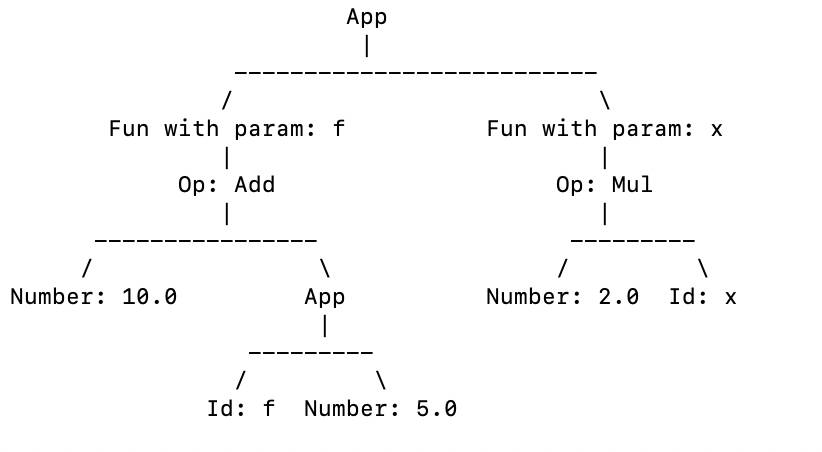
\includegraphics[width=\linewidth]{parseTreeViz.png}
\caption{Visualization of a parse tree generated using our parser and pretty-tree.\label{pretty-tree}}
\end{figure}

For the call tree, we would add numbers to each node with the provision of viewing the node's contents such as the environment.

\section{Goals}\label{stretch}
\subsection{Low-Risk Goals (100\%)}
\hl{Due to the technical difficulties in using ghc-vis, our low-risk goal will use only pretty-tree for visualization. Since the pretty-tree library does not have any features to help interact with the visualizations, the low-risk approach for the 100\% level will be to manually add more interactability to the call tree visualization, such as:}
        \begin{itemize}
            \item \hl{The ability to select a single node and view its details, such as its environment; and}
            \item \hl{The ability to search for and highlight in which nodes a certain identifier is bound.}
        \end{itemize}

\subsection{Stretch Goals (100\%+)}
There are a few ways to go above and beyond the scope of the current project:
\begin{itemize}
    \item Create separate implementations of parsing and visualizing FWAE for each new language feature addition in the course, i.e. first-class functions, followed by mutation, laziness, and recursion and the Y combinator.
        \begin{itemize}
            \item Mutation would be added to the language by altering the parser to parse \texttt{box}, \texttt{setbox!}, \texttt{unbox!}, and \texttt{set!}.
            \item Laziness would be implemented using thunks in the interpreter, and visualized lazily using ghc-vis' native lazy features.
            \item Recursive constructs would be added by altering the parser to parse \texttt{rec-with} and \texttt{rec-apply} using an implementation of the Y-combinator.
        \end{itemize}
    \item Get ghc-vis to work in GHCi via opening issues on its GitHub repository and reporting the bugs we've been experiencing.
    \item Create a custom interface for dynamically interacting with our parse and call trees, based on and possibly forking ghc-vis, altered to be tailored to our specific needs. An interface for inputting the FWAE code could also be added so that it does not have to be done via the REPL loop on the command line.
\end{itemize}

\begin{thebibliography}{99}

\bibitem{inclass6}
    CPSC 311 2018 WT1 staff.
    (2018).
    An interpreter with first-class functions via environments.
    In \textit{CPSC 311 Definition of Programming Languages: "Lambda Bound"}.
      \url{https://www.ugrad.cs.ubc.ca/~cs311/current/notes/in-class-06.rkt}.

\bibitem{fwae}
    \hl{
    Shriram Krishnamurthi.
    (26 April 2007).
    Programming Languages: Application and Interpretation.
    Retrieved 01 December 2018 from} \url{http://cs.brown.edu/~sk/Publications/Books/ProgLangs/2007-04-26/plai-2007-04-26.pdf}.

\bibitem{fwae-parser}
    Jonathan Chan, Ryan Chen, Samuel Or, and Megha Singhania.
    (9 November 2018).
    lmrjs/fwae-parser.
    In \textit{GitHub}.
    Retrieved 18 November 2018 from \url{https://github.com/lmrjs/fwae-parser/}.

\bibitem{parsec}
    Parsec contributors.
    (11 August 2018).
    haskell/parsec: A monadic parser combinator library.
    In \textit{GitHub}.
    Retrieved 13 November 2018, from \url{https://github.com/haskell/parsec}.
  
\bibitem{parsec-hackage}
    Daan Leijen and Paolo Martini.
    (2007).
    Text.Parsec.Prim.
    In \textit{Hackage}.
    Retrieved 18 November 2018 from \url{http://hackage.haskell.org/package/parsec-3.1.13.0/docs/Text-Parsec-Prim.html}.

\bibitem{lexer}
    Wikipedia contributors.
    (7 October 2018).
    Lexical analysis.
    In \textit{Wikipedia, The Free Encyclopedia}.
    Retrieved 18 November 2018 from \url{https://en.wikipedia.org/w/index.php?title=Lexical_analysis&oldid=862914890}.
    
\bibitem{parsec-bug}
    Mark Karpov.
    (15 April 2015).
    A possible bug in Text.Parsec.Token.float.
    In \textit{GitHub}.
    Retrieved 18 November 2018 from \url{https://github.com/haskell/parsec/issues/35#issuecomment-118612347}.
    
\bibitem{token}
    Herbert Valerio Riedel.
    (4 February 2018).
    parsec/Token.hs at master $\cdot$ haskell/parsec.
    In \textit{GitHub}.
    Retrieved 18 November 2018 from \url{https://github.com/haskell/parsec/blob/master/src/Text/Parsec/Token.hs#L568}.
    
\bibitem{ghc-vis}
    Felsing Dennis.
    (2012).
    The ghc-vis User Guide. 
    Retrieved 18 November 2018 from
      \url{https://lfelsin9.de/nnis/ghc-vis/}.
  
\bibitem{pretty-tree}
    Miljenovic Ivan.
    (2012).
    Drawing trees.
    Retrieved 21 November 2018 from
      \url{http://hackage.haskell.org/package/pretty-tree-0.1.0.0/docs/Data-Tree-Pretty.html}.
      
\bibitem{prelude}
    \hl{HaskellWiki contributors.
    (16 September 2008).
    Prelude.
    In \textit{HaskellWiki}.
    Retrieved 1 December 2018 from} \url{https://wiki.haskell.org/Prelude}.
      
\bibitem{data-tree}
    The University of Glasgow
    (2002).
    containers: Assorted concrete container types
    In \textit{Hackage}.
    Retrieved 21 November 2018 from \url{http://hackage.haskell.org/package/containers-0.6.0.1/docs/Data-Tree.html}.
\end{thebibliography}

\end{document}
